% Options for packages loaded elsewhere
\PassOptionsToPackage{unicode}{hyperref}
\PassOptionsToPackage{hyphens}{url}
\PassOptionsToPackage{dvipsnames,svgnames,x11names}{xcolor}
\documentclass[
  10pt,
  fontset=fandol]{ctexart}
\usepackage{xcolor}
\usepackage[margin=16mm]{geometry}
\usepackage{amsmath,amssymb}
\setcounter{secnumdepth}{-\maxdimen} % remove section numbering
\usepackage{iftex}
\ifPDFTeX
  \usepackage[T1]{fontenc}
  \usepackage[utf8]{inputenc}
  \usepackage{textcomp} % provide euro and other symbols
\else % if luatex or xetex
  \usepackage{unicode-math} % this also loads fontspec
  \defaultfontfeatures{Scale=MatchLowercase}
  \defaultfontfeatures[\rmfamily]{Ligatures=TeX,Scale=1}
\fi
\usepackage{lmodern}
\ifPDFTeX\else
  % xetex/luatex font selection
\fi
% Use upquote if available, for straight quotes in verbatim environments
\IfFileExists{upquote.sty}{\usepackage{upquote}}{}
\IfFileExists{microtype.sty}{% use microtype if available
  \usepackage[]{microtype}
  \UseMicrotypeSet[protrusion]{basicmath} % disable protrusion for tt fonts
}{}
\makeatletter
\@ifundefined{KOMAClassName}{% if non-KOMA class
  \IfFileExists{parskip.sty}{%
    \usepackage{parskip}
  }{% else
    \setlength{\parindent}{0pt}
    \setlength{\parskip}{6pt plus 2pt minus 1pt}}
}{% if KOMA class
  \KOMAoptions{parskip=half}}
\makeatother
\usepackage{longtable,booktabs,array}
\newcounter{none} % for unnumbered tables
\usepackage{calc} % for calculating minipage widths
% Correct order of tables after \paragraph or \subparagraph
\usepackage{etoolbox}
\makeatletter
\patchcmd\longtable{\par}{\if@noskipsec\mbox{}\fi\par}{}{}
\makeatother
% Allow footnotes in longtable head/foot
\IfFileExists{footnotehyper.sty}{\usepackage{footnotehyper}}{\usepackage{footnote}}
\makesavenoteenv{longtable}
\usepackage{graphicx}
\makeatletter
\newsavebox\pandoc@box
\newcommand*\pandocbounded[1]{% scales image to fit in text height/width
  \sbox\pandoc@box{#1}%
  \Gscale@div\@tempa{\textheight}{\dimexpr\ht\pandoc@box+\dp\pandoc@box\relax}%
  \Gscale@div\@tempb{\linewidth}{\wd\pandoc@box}%
  \ifdim\@tempb\p@<\@tempa\p@\let\@tempa\@tempb\fi% select the smaller of both
  \ifdim\@tempa\p@<\p@\scalebox{\@tempa}{\usebox\pandoc@box}%
  \else\usebox{\pandoc@box}%
  \fi%
}
% Set default figure placement to htbp
\def\fps@figure{htbp}
\makeatother
\setlength{\emergencystretch}{3em} % prevent overfull lines
\providecommand{\tightlist}{%
  \setlength{\itemsep}{0pt}\setlength{\parskip}{0pt}}
\usepackage{amsmath,amssymb,mathtools,needspace}
\xeCJKDeclareCharClass{CJK}{"2032,"0400->"04FF,"2160->"216B,"2460->"2473,"25A0,"25C7,"25CB,"25CF}
\IfFontExistsTF{Arial Unicode MS}{\xeCJKsetup{AutoFallBack=true}\setCJKfallbackfamilyfont{\CJKrmdefault}{Arial Unicode MS}}{}
\setcounter{secnumdepth}{0}
\setlength{\emergencystretch}{2em}
\allowdisplaybreaks
\usepackage{bookmark}
\IfFileExists{xurl.sty}{\usepackage{xurl}}{} % add URL line breaks if available
\urlstyle{same}
\hypersetup{
  pdftitle={快速算法设计:快速Walsh变换},
  colorlinks=true,
  linkcolor={Maroon},
  filecolor={Maroon},
  citecolor={Blue},
  urlcolor={Blue},
  pdfcreator={LaTeX via pandoc}}

\title{快速算法设计:快速Walsh变换}
\author{}
\date{}

\begin{document}
\maketitle

\section{*第 10 章　快速算法设计：快速 Walsh 变换}\label{ux7b2c-10-ux7ae0-ux5febux901fux7b97ux6cd5ux8bbeux8ba1ux5febux901f-walsh-ux53d8ux6362}

\subsection{10.1　美的 Walsh 函数}\label{ux7f8eux7684-walsh-ux51fdux6570}

随着大规模集成电路技术的广泛应用，信号普遍采取数字脉冲波形的形式。三角函数（即简谐波）不便于描述这类信号。为满足实际需要，人们考虑选用阶跃函数类的基函数。Walsh 函数就是阶跃函数类中一个完备的正交函数系。

Walsh 函数的一个显著特点是取值简单。它们仅取 \(+1\) 和 \(-1\) 两个值，因而可以方便地利用开关元件产生和处理数字信号。以 Walsh 函数为基底的线性变换称作 Walsh 变换。

与 Fourier 变换比较，Walsh 变换有其特点与优势。快速 Walsh 变换仅涉及加减运算而不含乘除操作，因而比快速 Fourier 变换更为迅捷。

Walsh 分析有着深刻的内涵。20 世纪 70 年代初，著名应用数学家 Harmuth 曾惊人地预言：\textbf{Walsh 分析的研究将导致一场数学革命，就像 17、18 世纪的微积分那样。}

这是一场什么样的``数学革命''呢？

\subsubsection{10.1.1　微积分的逼近法}\label{ux5faeux79efux5206ux7684ux903cux8fd1ux6cd5}

经典数学的基础是微积分。从微积分的观点看，在一切函数中，以多项式最为简单。能否用简单的多项式来逼近一般函数呢？众所周知的 Taylor 分析（1715 年）肯定了这一事实。Taylor 级数

\[
f(x)\sim\sum_{k=0}^{\infty}\frac{f^{(k)}(x_0)}{k!}(x-x_0)^k
\]

表明，一般的光滑函数 \(f(x)\) 可用多项式来近似地刻画。Taylor 分析是 18 世纪初的一项重大的数学成就。

然而 Taylor 分析存在严重的缺陷：它的条件很苛刻，要求 \(f(x)\) 足够光滑并提供出它的各阶导数值 \(f^{(k)}(x_0)\)；此外，Taylor 分析的整体逼近效果差，它仅能保证在展开点 \(x_0\) 的某个邻域内有效。

时移物换，百年之后 Fourier（1822 年）指出，``任何函数，无论怎样复杂，均可表示为三角级数的形式''：

\href{../../source-images/pdf-262.jpeg}{原页}

\[
f(x)\sim\frac{a_0}{2}+\sum_{k=1}^{\infty}(a_k\cos2\pi kx+b_k\sin2\pi kx),\quad 0\leqslant x<1.
\]

这就是今日被称作``Fourier 分析''的数学方法。著名数学家 M. Kline 评价这一数学成就是``19 世纪数学的第一大步，并且是真正极为重要的一步''。

Fourier 关于任意函数都可以表达为三角级数这一思想被誉为``数学史上最大胆，最辉煌的概念''。

Fourier 的成就使人们从 Taylor 分析的理想函数类中解放出来。Fourier 分析不仅放宽了光滑性的限制，还保证了整体的逼近效果。

从数学美的角度来看，Fourier 分析也比 Taylor 分析更美，其基函数系------三角函数系是个完备的正交函数系。尤其值得注意的是，这个函数系可以视作是由一个简单函数 \(\cos x\) 经过简单的伸缩平移变换加工生成的。Fourier 分析表明，任何复杂函数都可以借助于简单函数 \(\cos x\) 来刻画，即

\[
\cos x\xrightarrow{\text{伸缩＋平移}}\text{三角函数系}\xrightarrow{\text{组合}}\text{任意函数 }f(x).
\]

这是一个惊人的事实。在这里，被逼近函数 \(f(x)\) 的``繁''与逼近工具 \(\cos x\) 的``简''两者反差很大，因此 Fourier 逼近很美。Fourier 分析在数学史上被誉``一首数学的诗''，Fourier 则有``数学诗人''的美称。

\subsubsection{10.1.2　Walsh 函数的复杂性}\label{walsh-ux51fdux6570ux7684ux590dux6742ux6027}

1923 年，美国数学家 J. L. Walsh 又提出了一个完备的正交函数系，后人将其称作 Walsh 函数系。第 \(k\) 族 Walsh 函数含有 \(2^k\) 个函数，其中第 \(i\) 个函数 \(W_{ki}\) 有如下解析表达式：

\[
\begin{gathered}
W_{ki}(x)=\prod_{r=0}^{k-1}\operatorname{sgn}[\cos i_r2^r\pi x],\quad 0\leqslant x<1,\\
k=0,1,2,\cdots,\quad i=0,1,\cdots,2^k-1,
\end{gathered}
\]

式中，\(\operatorname{sgn}\) 是\textbf{符号函数}，当 \(x\geqslant0\) 时 \(\operatorname{sgn}[x]\) 取值 \(+1\)，而 \(x<0\) 时取值 \(-1\)。又 \(i_r\) 取值 \(0\) 或 \(1\) 是序数 \(i\) 的二进制码：

\[
i=\sum_{r=0}^{k-1}i_r2^r.
\]

图 10.1 列出前面 16 个 Walsh 函数的波形。其中，第 1 个（标号 0）组成第 0 族，前两个（标号 0 与 1）组成第 1 族；前 4 个（标号 0、1、2、3）组成第 2 族，依此类推，前 16 个组成第 4 族 Walsh 函数。

Walsh 函数取值简单，它们仅取 \(\pm1\) 两个值，但其波形却很复杂，似乎比三角函数要复杂得多，以致依据定义很难作出它们的图形。

由于表达式中含有符号运算 \(\operatorname{sgn}\)，Walsh 函数的波形频繁起伏，甚至``几乎处处''不连续（见图 10.1），经典的微积分方法在这里难以施展身手，Walsh 函数系的形态

\href{../../source-images/pdf-263.jpeg}{原页}

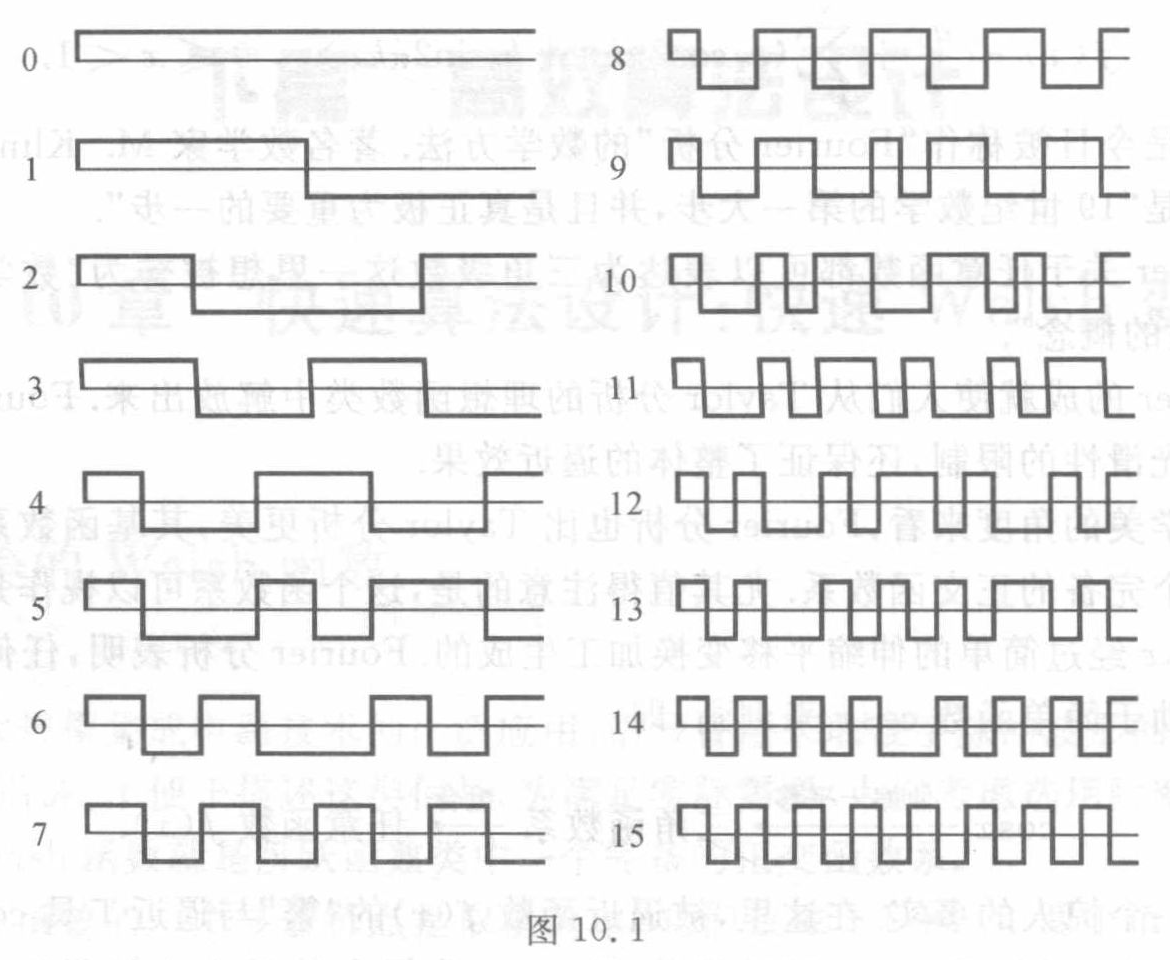
\includegraphics[width=0.85\linewidth,height=\textheight,keepaspectratio,alt={图 10.1（原图裁切）：前 16 个 Walsh 函数的波形}]{../assets/ch10/fig-10-1.png}

图 10.1

\begin{quote}
图中文字与图意（转录）：左列波形标号依次为 0、1、2、3、4、5、6、7，右列依次为 8、9、10、11、12、13、14、15。各条波形在水平基线上下取两个阶跃值；标号 0 的波形为方波。
\end{quote}

怪异与表达式复杂使人们对它望而却步，在提出后的许多年里，它一直默默无闻，不被人们所重视。

直到 20 世纪 60 年代末，人们才惊异地发现，Walsh 函数可应用于信号处理的众多领域，诸如通信、声呐、雷达、图像处理、语音识别、遥感遥测遥控、仪表、医学、天文、地质等等。

``真''是``美''的反光。有着广泛应用的 Walsh 函数美在哪里呢？

\subsubsection{10.1.3　Walsh 分析的数学美}\label{walsh-ux5206ux6790ux7684ux6570ux5b66ux7f8e}

后文将揭示出一个惊人的事实：表面看起来极其复杂的 Walsh 函数系，竟然是由一个简单得不能再简单的方波 \(R(x)=1\) 演化生成的。实际上，从方波 \(R(x)\) 出发，经过伸缩、平移的二分手续，即可演化生成 Walsh 函数系。Walsh 函数系是个完备的正交函数系，它可以用来逼近一般的复杂函数。这样，Walsh 逼近有下述路线图：

\[
R(x)=1\xrightarrow[\text{（二分手续）}]{\text{伸缩＋平移}}\text{Walsh 函数系}\xrightarrow{\text{组合}}\text{复杂函数 }f(x).
\]

与 Fourier 分析相比，Walsh 分析更为简洁，它表明：在某种意义上，任何复杂函数 \(f(x)\) 都是简单的方波 \(R(x)=1\) 二分演化的结果。

综上所述，数学史上近三个世纪提出的三种逼近方法，即 18 世纪初（1715 年）的 Taylor 分析、19 世纪初（1822 年）的 Fourier 分析和 20 世纪初（1923 年）的 Walsh 分析，它们都是数学美的光辉典范，是``百年绝唱三首数学诗''。

这些逼近工具一个比一个更美。Fourier 分析具有深度的数学美，而 Walsh 分析

\href{../../source-images/pdf-264.jpeg}{原页}

则具有极度的数学美。

问题在于，为了撩开 Walsh 函数玄妙而神秘的面纱，必须换一种思维方式进行考察。

\subsection{10.2　Walsh 函数代数化}\label{walsh-ux51fdux6570ux4ee3ux6570ux5316}

本节将限定在区间 \([0,1)\) 上考察 Walsh 函数。由于自变量 \(x\) 在实际应用中通常代表时间，因此称区间 \([0,1)\) 为\textbf{时基}。

\subsubsection{10.2.1　时基上的二分集}\label{ux65f6ux57faux4e0aux7684ux4e8cux5206ux96c6}

由图 10.1 可以看出，Walsh 函数是时基上的阶跃函数，每个 Walsh 函数在给定分划的每个子段上取定值 \(+1\) 或 \(-1\)。怎样刻画 Walsh 函数所依赖的分划呢？

为便于刻画 Walsh 函数的跃变特征，首先引进二分集的概念。设将时基 \(E_1=[0,1)\) 对半二分，其左右两个子段合并为集 \(E_2\)，即

\[
E_2=\left[0,\frac12\right)\cup\left[\frac12,1\right).
\]

再将 \(E_2\) 的每个子段对半二分，又得含有 4 个子段的区间集 \(E_4\)，即

\[
E_4=\left[0,\frac14\right)\cup\left[\frac14,\frac12\right)\cup\left[\frac12,\frac34\right)\cup\left[\frac34,1\right).
\]

如此二分下去，二分 \(n\) 次所得的区间集含有 \(N=2^n\) 个子段，即

\[
E_N=\bigcup_{i=0}^{N-1}\left[\frac{i}{N},\frac{i+1}{N}\right),\quad n=0,1,2,\cdots.
\]

这样得出的区间集 \(E_N\)，\(N=1,2,4,\cdots\) 称作时基上的\textbf{二分集}（见图 10.2）。

在二分集的每个子段上取定值的函数称作二分集上的\textbf{阶跃函数}。阶跃函数在某一子段上的函数值称作\textbf{阶跃值}。

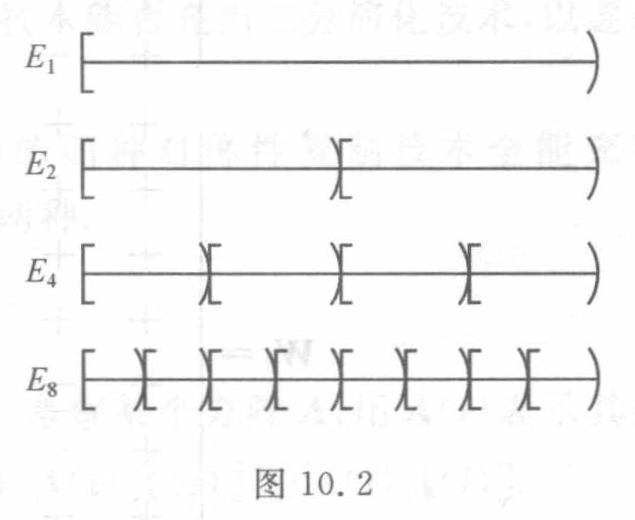
\includegraphics[width=0.85\linewidth,height=\textheight,keepaspectratio,alt={图 10.2（原图裁切）：时基上的二分集}]{../assets/ch10/fig-10-2.png}

图 10.2

\begin{quote}
图中文字与图意（转录）：四行标号为 \(E_1\)、\(E_2\)、\(E_4\)、\(E_8\)，每行表示左闭右开的子段，按行依次二分。
\end{quote}

现在的问题是，如何在二分集的各个子段上布值 \(+1\) 与 \(-1\) 以设计出一个完备的正交函数系？实际上，这种函数系就是 Walsh 函数系。

为规范起见，约定 Walsh 函数第一个阶跃值（即最左侧的子段上的函数值）为 \(+1\)，如图 10.1 所示。

在形形色色的 Walsh 函数中，最简单的自然是\textbf{方波}

\[
R(x)=1,\quad0\leqslant x<1.
\]

然而这个函数过于平凡而显得``空虚''，其中似乎不含任何信息。``波''的含义是波动、起伏。按这种理解，时基上的方波似乎不能算作真正的``波''。具有波动性的最简单的

\href{../../source-images/pdf-265.jpeg}{原页}

波形是下列 \textbf{Haar 波}：

\[
H(x)=\begin{cases}
+1,&0\leqslant x<\dfrac12,\\[4pt]
-1,&\dfrac12\leqslant x<1.
\end{cases}
\]

由图 10.1 知，方波与 Haar 波是 Walsh 函数系的源头。

\subsubsection{10.2.2　Walsh 函数的矩阵表示}\label{walsh-ux51fdux6570ux7684ux77e9ux9635ux8868ux793a}

Walsh 函数仅取 \(+1\) 与 \(-1\) 两个值。为简约起见，后文常将 \(+1\) 与 \(-1\) 简记为``\(+\)''与``\(-\)''。

由于 Walsh 函数在二分集的每个子段上取值 \(+\) 或 \(-\)，因而它们可表示为某个向量，而第 \(n\) 族 Walsh 函数的全体则可表达为一个 \(N=2^n\) 阶方阵，称作 \textbf{Walsh 方阵}。

据图 10.1 容易看出，前面几个 Walsh 方阵分别是

\[
W_1=[\,+\,],
\]

\[
W_2=\begin{pmatrix}+&+\\+&-\end{pmatrix},
\]

\[
W_4=\begin{pmatrix}
+&+&+&+\\
+&+&-&-\\
+&-&-&+\\
+&-&+&-
\end{pmatrix},
\]

\[
W_8=\begin{pmatrix}
+&+&+&+&+&+&+&+\\
+&+&+&+&-&-&-&-\\
+&+&-&-&-&-&+&+\\
+&+&-&-&+&+&-&-\\
+&-&-&+&+&-&-&+\\
+&-&-&+&-&+&+&-\\
+&-&+&-&-&+&-&+\\
+&-&+&-&+&-&+&-
\end{pmatrix}.
\]

请读者据图 10.1 列出 Walsh 方阵 \(W_{16}\)。

Walsh 方阵看上去是个复杂系统，这个复杂系统中究竟潜藏着怎样的规律性呢？

\subsection{10.3　Walsh 阵的二分演化}\label{walsh-ux9635ux7684ux4e8cux5206ux6f14ux5316}

现在的问题是，能否设计出某种简单的二分手续，以将方波 \(W_1=[+]\) 逐步演化

\href{../../source-images/pdf-266.jpeg}{原页}

生成各阶 Walsh 方阵，即

\[
W_1\Rightarrow W_2\Rightarrow W_4\Rightarrow W_8\Rightarrow\cdots.
\]

这里箭头``\(\Rightarrow\)''表示所要设计的二分演化手续。

二分手续应当是简单而有效的。对于矩阵演化，什么样的演化手续最为简单呢？

\subsubsection{10.3.1　矩阵的对称性复制}\label{ux77e9ux9635ux7684ux5bf9ux79f0ux6027ux590dux5236}

就矩阵演化来说，最为简单的演化手续是对称性复制。这种演化手续易于在计算机上实现，而且有丰富的文化内涵。

大自然的基本设计是美的，美意味着简单，美意味着对称。本节所考察的对称性分镜像对称与平移对称两种，它们在某种意义上互为反对称。镜像对称又分偶对称与奇对称，平移对称又分正对称与反对称。此外，矩阵的复制对象分矩阵行与矩阵块两种情况，这样，Walsh 方阵的对称性复制可考虑表 10.1 所列的四种方案。

表 10.1

{\def\LTcaptype{none} % do not increment counter
\begin{longtable}[]{@{}lll@{}}
\toprule\noalign{}
对称性 & 复制对象：矩阵行 & 复制对象：矩阵块 \\
\midrule\noalign{}
\endhead
\bottomrule\noalign{}
\endlastfoot
镜像对称 & 镜像行复制 & 镜像块复制 \\
平移对称 & 平移行复制 & 平移块复制 \\
\end{longtable}
}

人们自然关心，矩阵的上述几种对称性复制技术能否充当二分演化技术，以逐步演化生成各种 Walsh 方阵呢？

答案是令人振奋的。事实上，表 10.1 所列的四种对称性复制技术全能充当 Walsh 演化的二分手续。后文将着重考察其中的两种。

\subsubsection{10.3.2　Walsh 阵的演化生成}\label{walsh-ux9635ux7684ux6f14ux5316ux751fux6210}

首先考察表 10.1 中镜像行复制的演化方式。考察某个方阵 \(A\)，用 \(A(i)\) 表示其第 \(i\) 行，对 \(A(i)\) 施行偶复制与奇复制，分别生成向量 \([A(i)\mathrel{\vdots}\ddot A(i)]\) 与 \([A(i)\mathrel{\vdots}\dot A(i)]\)。

例如，设 \(A(i)=[+\ -]\)，则

\[
[A(i)\mathrel{\vdots}\ddot A(i)]=[+\ -\mathrel{\vdots}-\ +],
\]

\[
[A(i)\mathrel{\vdots}\dot A(i)]=[+\ -\mathrel{\vdots}+\ -].
\]

进一步，若 \(A(i)=[+\ -\mathrel{\vdots}+\ -]\)，则

\[
[A(i)\mathrel{\vdots}\ddot A(i)]=[+\ -\ +\ -\mathrel{\vdots}-\ +\ -\ +],
\]

\[
[A(i)\mathrel{\vdots}\dot A(i)]=[+\ -\ +\ -\mathrel{\vdots}+\ -\ +\ -].
\]

如果对方阵 \(A\) 的每一行先后施行偶复制与奇复制两种复制手续，即可生成一个阶数倍增的方阵 \(B\)，这种演化手续称作\textbf{镜像行复制}，即

\href{../../source-images/pdf-267.jpeg}{原页}

\[
A=\begin{pmatrix}\vdots\\A(i)\\\vdots\end{pmatrix}
\longrightarrow B=\begin{pmatrix}
\vdots\\
A(i)\mathrel{\vdots}\ddot A(i)\\
A(i)\mathrel{\vdots}\dot A(i)\\
\vdots
\end{pmatrix}.
\]

人们自然会问，如果对方波 \([+]\) 反复施行镜像行复制的演化手续，使其阶数逐步倍增，将会生成什么样的方阵序列呢？

1 阶方阵 \([+]\) 仅有一行（一列），对它施行偶复制与奇复制，分别生成 \([+\mathrel{\vdots}+]\) 与 \([+\mathrel{\vdots}-]\)，两者合成在一起，结果生成一个 2 阶方阵

\[
[+]\longrightarrow\begin{pmatrix}+&+\\+&-\end{pmatrix}.
\]

对所生成的 2 阶方阵的两行 \([+\ +]\) 与 \([+\ -]\) 分别施行镜像复制的偶复制与奇复制，进一步生成一个 4 阶方阵

\[
\begin{pmatrix}+&+\\+&-\end{pmatrix}\longrightarrow
\begin{pmatrix}
+&+&+&+\\
+&+&-&-\\
+&-&-&+\\
+&-&+&-
\end{pmatrix}.
\]

继续对所生成的 4 阶方阵施行镜像行复制，获得如下 8 阶方阵，即

\[
\begin{pmatrix}
+&+&+&+\\
+&+&-&-\\
+&-&-&+\\
+&-&+&-
\end{pmatrix}\longrightarrow
\begin{pmatrix}
+&+&+&+&+&+&+&+\\
+&+&+&+&-&-&-&-\\
+&+&-&-&-&-&+&+\\
+&+&-&-&+&+&-&-\\
+&-&-&+&+&-&-&+\\
+&-&-&+&-&+&+&-\\
+&-&+&-&-&+&-&+\\
+&-&+&-&+&-&+&-
\end{pmatrix}.
\]

上述方阵与 10.2.2 小节列出的 Walsh 方阵相比较，两者完全一致。可以证明，从方波 \([+]\) 出发，运用镜像行复制的演化技术可以生成 Walsh 方阵序列。这个 Walsh 方阵等价于 10.1.2 小节的原始定义。

Walsh 方阵有多种排序方式。镜像行复制生成的 Walsh 方阵特别称作 \textbf{Walsh 阵}。

\subsubsection{10.3.3　Walsh 阵的演化机制}\label{walsh-ux9635ux7684ux6f14ux5316ux673aux5236}

Walsh 阵的演化方式从属于二分演化模式。事实上，这里从初态 \(W_1=[+]\) 出发，将 \(W_{N/2}\) 加工成 \(W_N\) 的二分手续如下。

（1）分裂手续。

\href{../../source-images/pdf-268.jpeg}{原页}

对 \(W_{N/2}\) 的每一行 \(W_{N/2}(i)\) 分别施行偶复制与奇复制，生成两个 \(N\) 维向量 \([W_{N/2}(i)\mathrel{\vdots}\ddot W_{N/2}(i)]\) 与 \([W_{N/2}(i)\mathrel{\vdots}\dot W_{N/2}(i)]\)。

（2）合成手续。

将 \(W_{N/2}\) 的每一行按上述分裂手续扩展为相邻的两个 \(N\) 维向量，从而将 \(W_{N/2}\) 扩展成为一个 \(N\) 阶方阵

\[
W_N=\begin{pmatrix}
\vdots&\vdots\\
W_{N/2}(i)\mathrel{\vdots}&\ddot W_{N/2}(i)\\
W_{N/2}(i)\mathrel{\vdots}&\dot W_{N/2}(i)\\
\vdots&\vdots
\end{pmatrix},
\]

如此反复地做下去。这种二分演化机制如图 10.3 所示。如 10.1.2 小节所看到的，Walsh 函数的表达式很复杂，直接利用表达式生成 Walsh 函数很困难。然而依据上述镜像行复制的演化方式，一蹴而就地派生出一个又一个 Walsh 方阵，从而得到一族又一族 Walsh 函数。Walsh 函数的数目是逐族倍增的，这是一种快速生成算法。

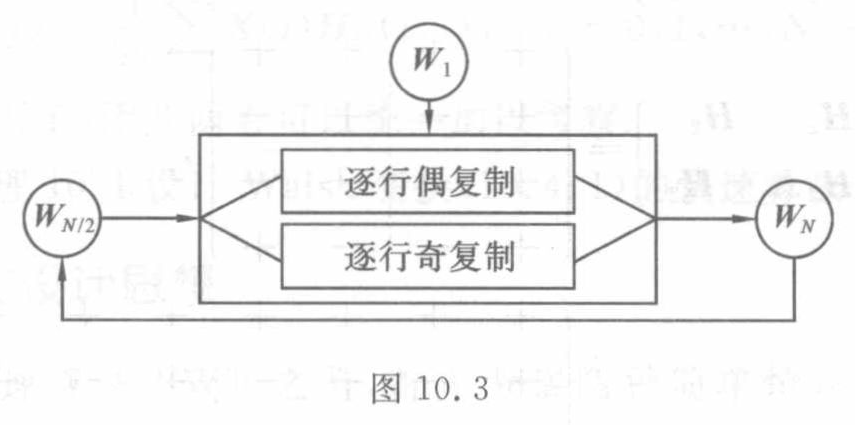
\includegraphics[width=0.85\linewidth,height=\textheight,keepaspectratio,alt={图 10.3（原图裁切）：Walsh 阵的二分演化机制}]{../assets/ch10/fig-10-3.png}

图 10.3

\begin{quote}
图中文字与图意（转录）：初态 \(W_1\) 从上方进入；\(W_{N/2}\) 分成``逐行偶复制''和``逐行奇复制''两路，合成为 \(W_N\)；\(W_N\) 经下方反馈线返回 \(W_{N/2}\)。
\end{quote}

\subsubsection{10.3.4　Hadamard 阵的演化生成}\label{hadamard-ux9635ux7684ux6f14ux5316ux751fux6210}

上述镜像行复制的演化方式能否进一步简化呢？

从研究者的角度来说，平移对称比镜像对称更易于接受，而矩阵块比矩阵行更易于把握，现在进一步考察表 10.1 所列的平移块复制的演化方式。

考察某个方阵 \(A\)，直接对它施行平移正复制与平移反复制，分别生成 \([A\mathrel{\vdots}A]\) 与 \([A\mathrel{\vdots}-A]\)，两者合成在一起，得阶数倍增的方阵

\[
B=\begin{pmatrix}A&A\\A&-A\end{pmatrix}.
\]

这种演化方式称作\textbf{平移块复制}。

仍然从方波 \([+]\) 出发，反复施行平移块复制的演化方式，所生成的一系列方阵称作 \textbf{Hadamard 阵}。\(N\) 阶 Hadamard 阵记作 \(H_N\)。特别地，\(H_1=[+]\)。

显然，Hadamard 阵的演化机制同样从属于二分演化模式，如图 10.4 所示。

按平移块复制的演化方式，如果将 \(H_N\) 对分为 4 块，则其左上、右上与左下三块均为 \(H_{N/2}\)，而其右下则为 \(-H_{N/2}\)，即 Hadamard 阵有形式简单的递推表达式

\href{../../source-images/pdf-269.jpeg}{原页}

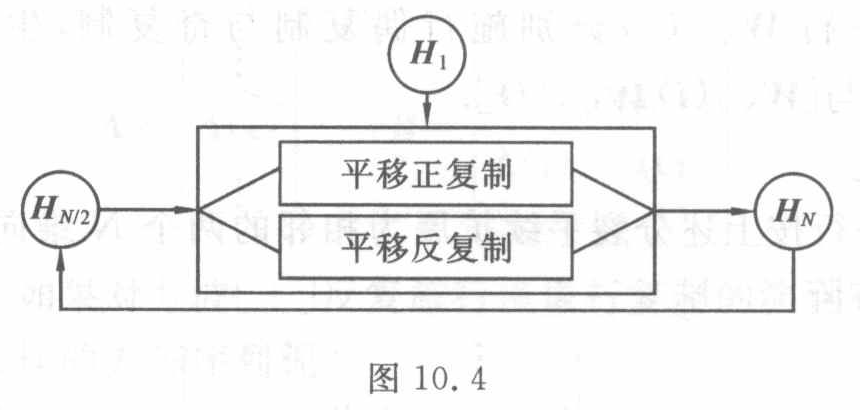
\includegraphics[width=0.85\linewidth,height=\textheight,keepaspectratio,alt={图 10.4（原图裁切）：Hadamard 阵的二分演化机制}]{../assets/ch10/fig-10-4.png}

图 10.4

\begin{quote}
图中文字与图意（转录）：初态 \(H_1\) 从上方进入；\(H_{N/2}\) 分成``平移正复制''和``平移反复制''两路，合成为 \(H_N\)；\(H_N\) 经下方反馈线返回 \(H_{N/2}\)。
\end{quote}

\[
H_N=\begin{pmatrix}H_{N/2}&H_{N/2}\\H_{N/2}&-H_{N/2}\end{pmatrix},\quad N=2,4,8,\cdots.
\tag{10.3.1}
\]

可见，Hadamard 阵的演化过程是简单的。事实上，从方波 \([+]\) 出发，按式（10.3.1）反复施行演化手续，有

\[
H_1=[+],
\]

\[
H_2=\begin{pmatrix}H_1&H_1\\H_1&-H_1\end{pmatrix}=\begin{pmatrix}+&+\\+&-\end{pmatrix},
\]

\[
H_4=\begin{pmatrix}H_2&H_2\\H_2&-H_2\end{pmatrix}=\begin{pmatrix}
+&+&+&+\\
+&-&+&-\\
+&+&-&-\\
+&-&-&+
\end{pmatrix},
\]

\[
H_8=\begin{pmatrix}H_4&H_4\\H_4&-H_4\end{pmatrix}=\begin{pmatrix}
+&+&+&+&+&+&+&+\\
+&-&+&-&+&-&+&-\\
+&+&-&-&+&+&-&-\\
+&-&-&+&+&-&-&+\\
+&+&+&+&-&-&-&-\\
+&-&+&-&-&+&-&+\\
+&+&-&-&-&-&+&+\\
+&-&-&+&-&+&+&-
\end{pmatrix}.
\]

如此继续下去，可以证明，这样演化生成的 Hadamard 阵同样是一种 Walsh 方阵。这里的 Hadamard 阵同 Walsh 阵相比较，两者只是行（列）的排序方式不同而已。

进一步考察矩阵元素的递推关系。前已指出，如果将矩阵 \(H_N\) 对分为 4 块，则其左上、右上与左下 3 块均为 \(H_{N/2}\)，而右下块则为 \(-H_{N/2}\)。记 \(H_N(i,j)\) 为矩阵 \(H_N\) 第 \(i\) 行第 \(j\) 列的元素，则上下两组\textbf{平移对} \((i,j)\)、\((i,N/2+j)\) 与 \((N/2+i,j)\)、\((N/2+i,N/2+j)\) 的矩阵元素有定理 10.1 所述的关系。

\textbf{定理 10.1}　对于 \(0\leqslant i,j\leqslant N/2-1\)，有

\[
\begin{aligned}
H_N(i,j)&=H_N(i,N/2+j)=H_N(N/2+i,j)\\
&=-H_N(N/2+i,N/2+j)=H_{N/2}(i,j).
\end{aligned}
\]

\href{../../source-images/pdf-270.jpeg}{原页}

现在基于 Hadamard 阵的上述表达式设计 Walsh 变换的快速算法 FWT。FWT 的设计同样从属于二分演化模式。

\subsection{10.4　快速变换 FWT}\label{ux5febux901fux53d8ux6362-fwt}

不同排序方式的 Walsh 变换，其快速算法的设计方法彼此类同。本节将着重考察 Hadamard 序的 Walsh 变换 \(N\)-WT

\[
X(i)=\sum_{j=0}^{N-1}x(j)H_N(i,j),\quad i=0,1,\cdots,N-1,
\tag{10.4.1}
\]

式中，\(H_N\) 为 \(N\) 阶 Hadamard 阵，\(\{x(j)\}_0^{N-1}\) 为输入数据，输出数据 \(\{X(i)\}_0^{N-1}\) 待求。这里仍然假定 \(N=2^n\)，\(n\) 为正整数。

由于 Hadamard 阵是对称正交阵，Walsh 变换（10.4.1）同它的逆变换

\[
x(j)=\frac1N\sum_{i=0}^{N-1}X(i)H_N(i,j),\quad j=0,1,\cdots,N-1
\]

仅仅相差一个常数因子，因此两者可以统一加以考察。

本节将基于定理 10.1 设计 Walsh 变换（10.4.1）的快速算法 FWT。

\begin{quote}
校注（agent 补充，CH10-E002）：原文``对称正交阵''照录。依本章未归一化的 \(\pm1\) 元素定义，\(H_N^\mathsf{T}H_N=NI\)，\(N>1\) 时并非通常定义下满足 \(Q^\mathsf{T}Q=I\) 的正交矩阵；准确地说其行列两两正交，\(H_N/\sqrt N\) 才是正交矩阵。原页逆变换中的 \(1/N\) 因子与该定义一致。本项是原书术语疑误，不是 OCR 错误。
\end{quote}

\subsubsection{10.4.1　FWT 的设计思想}\label{fwt-ux7684ux8bbeux8ba1ux601dux60f3}

在具体设计快速算法 FWT 之前，首先考察两种简单情形。由于 1 阶和 2 阶 Hadamard 阵为

\[
H_1=[\,+\,],
\]

\[
H_2=\begin{pmatrix}+&+\\+&-\end{pmatrix},
\]

因而 1-WT 具有极其简单的形式

\[
X(0)=x(0).
\]

这里输入数据即为所求结果，因而不需要做任何计算。此外，2-WT 为

\[
\begin{cases}
X(0)=x(0)+x(1),\\
X(1)=x(0)-x(1).
\end{cases}
\]

这项计算也很平凡，不存在算法设计问题。

可见，1-WT 与 2-WT 都是极为简单的。

\textbf{快速算法 FWT 的设计思想是，基于规模减半的二分手续，通过 2-WT 的反复计算，将所给 \(N\)-WT 逐步加工成 1-WT，从而得出所求的结果。}

快速算法 FWT 是优秀算法的一朵奇葩，它鲜明地展现了``简单的重复生成复杂''这一算法设计的基本理念。此外，它可以充当一个样板，示范运用二分演化机制设

\href{../../source-images/pdf-271.jpeg}{原页}

计快速变换的全过程。

\subsubsection{10.4.2　FWT 的演化机制}\label{fwt-ux7684ux6f14ux5316ux673aux5236}

前已反复指出，二分技术是快速算法设计的基本技术。二分技术的基本点是运用某种二分手续，将所给计算问题化归为规模减半的同类问题。

对于 \(N\) 点 Walsh 变换 \(N\)-WT（10.4.1），即

\[
X(i)=\sum_{j=0}^{N-1}x(j)H_N(i,j),\quad i=0,1,\cdots,N-1.
\]

将其右端的和式对半拆开，有

\[
\begin{aligned}
X(i)&=\sum_{j=0}^{N/2-1}x(j)H_N(i,j)+\sum_{j=N/2}^{N-1}x(j)H_N(i,j)\\
&=\sum_{j=0}^{N/2-1}[x(j)H_N(i,j)+x(N/2+j)H_N(i,N/2+j)],\quad i=0,1,\cdots,N-1.
\end{aligned}
\]

然后再将这组算式对半分为两组算式，有

\[
\begin{cases}
\displaystyle X(i)=\sum_{j=0}^{N/2-1}[x(j)H_N(i,j)+x(N/2+j)H_N(i,N/2+j)],\\[6pt]
\displaystyle X(N/2+i)=\sum_{j=0}^{N/2-1}[x(j)H_N(N/2+i,j)+x(N/2+j)H_N(N/2+i,N/2+j)],
\end{cases}
\]

\[
i=0,1,\cdots,N/2-1.
\]

利用定理 1 的递推关系将上述算式化简，得

\[
\begin{cases}
\displaystyle X(i)=\sum_{j=0}^{N/2-1}[x(j)+x(N/2+j)]H_{N/2}(i,j),\\[6pt]
\displaystyle X(N/2+i)=\sum_{j=0}^{N/2-1}[x(j)-x(N/2+j)]H_{N/2}(N/2+i,j),
\end{cases}\quad i=0,1,\cdots,N/2-1.
\]

这样，所给 \(N\)-WT（10.4.1）被加工成下列两个 \(N/2\)-WT：

\[
\begin{cases}
\displaystyle X(i)=\sum_{j=0}^{N/2-1}x_1(j)H_{N/2}(i,j),\\[6pt]
\displaystyle X(N/2+i)=\sum_{j=0}^{N/2-1}x_1(N/2+j)H_{N/2}(N/2+i,j),
\end{cases}\quad i=0,1,\cdots,N/2-1.
\]

为此所要施行的二分手续是

\[
\begin{cases}
x_1(j)=x(j)+x(N/2+j),\\
x_1(N/2+j)=x(j)-x(N/2+j),
\end{cases}\quad j=0,1,\cdots,N/2-1
\tag{10.4.2}
\]

上述二分手续将所给 \(N\)-WT 加工成 2 个 \(N/2\)-WT。每个 \(N/2\)-WT 通过二分手续可进一步加工成 2 个 \(N/4\)-WT。如此反复二分，使问题的规模逐次减半，最终可将

\begin{quote}
校注（agent 补充，CH10-E001）：本页化简式及其后两个 \(N/2\)-WT 的第二式，原图均写作 \(H_{N/2}(N/2+i,j)\)，上文已照录。按前页定理 10.1 和本章对 \(N/2\) 阶矩阵的索引范围，这里的行指标 \(N/2+i\) 超出 \(0,\ldots,N/2-1\)；由 \(H_N(N/2+i,j)=H_{N/2}(i,j)\)，两处应为 \(H_{N/2}(i,j)\)。这是原书下标疑误，不是 OCR 错误。\href{../assets/ch10/erratum-p271-indices.png}{原式放大裁片}。此外，本页``定理 1''照录，所用递推关系对应前页``定理 10.1''。
\end{quote}

\href{../../source-images/pdf-272.jpeg}{原页}

\(N\)-WT 加工成 \(N\) 个 1-WT，从而得出所求的结果。这种演化过程

\[
\underset{\text{（计算模型）}}{N\text{-WT}}\Rightarrow2\text{ 个 }N/2\text{-WT}\Rightarrow4\text{ 个 }N/4\text{-WT}\Rightarrow\cdots\Rightarrow\underset{\text{（计算结果）}}{N\text{ 个 }1\text{-WT}}
\]

称作\textbf{快速 Walsh 变换}。这里箭头``\(\Rightarrow\)''表示二分手续（10.4.2）。

进一步剖析二分手续（10.4.2）的内涵，计算模型 \(N\)-WT 所要加工的数据 \(\{x(j)\}\) 是个 \(N\) 维向量，将它对半二分，得 \(N/2\) 个\textbf{平移对} \((x(j),x(N/2+j))\)。可见二分手续（10.4.2）的含义是，将平移对的两个数据相加减，因而 FWT 从属于图 10.5 的二分演化模式。

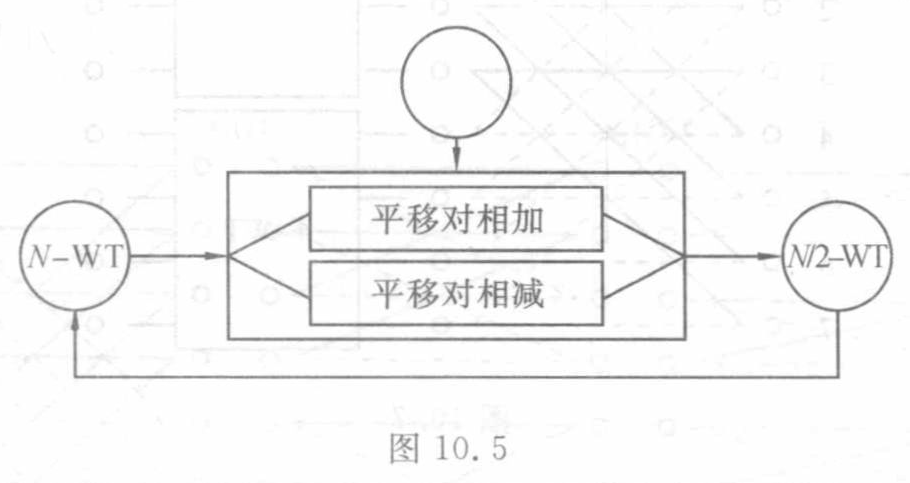
\includegraphics[width=0.85\linewidth,height=\textheight,keepaspectratio,alt={图 10.5（原图裁切）：FWT 的二分演化模式}]{../assets/ch10/fig-10-5.png}

图 10.5

\begin{quote}
图中文字与图意（转录）：左端 \(N\)-WT 进入``平移对相加''和``平移对相减''两路，合成右端 \(N/2\)-WT，底部有返回左端的反馈线；顶部有一个向下接入的空圆，原图未印文字标签。
\end{quote}

最后统计 FWT 的运算量。由于 FWT 的每一步使问题的的规模减半，欲将所给 \(N\)-WT，\(N=2^n\) 加工成 \(N\) 个 1-WT，二分演化需做 \(n=\log_2N\) 步，又形如式（10.4.2）的二分手续的每一步要做 \(N\) 次加减操作，因而 FWT 的总运算量为 \(N\log_2N\) 次加减操作。另一方面，如果直接计算 \(N\)-WT（10.4.1）要做 \(N^2\) 次加减操作，故 FWT 是快速算法，其加速比

\[
\frac{N^2}{N\log_2N}\to\infty\quad\text{（当 }N\to\infty\text{ 时）}.
\]

\subsubsection{10.4.3　FWT 的计算流程}\label{fwt-ux7684ux8ba1ux7b97ux6d41ux7a0b}

二分手续（10.4.2）采取两两加工的处理方式，即将一对数据 \((x(j),x(N/2+j))\) 加工成一对新的数据 \((x_1(j),x_1(N/2+j))\)，其计算格式如图 10.6 所示。这里分别用实线与虚线区分数据的相加与相减两种运算。

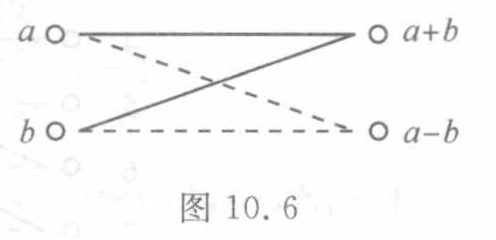
\includegraphics[width=0.85\linewidth,height=\textheight,keepaspectratio,alt={图 10.6（原图裁切）：两两加工的计算格式}]{../assets/ch10/fig-10-6.png}

图 10.6

\begin{quote}
图中文字与图意（转录）：左端输入从上到下为 \(a\)、\(b\)，右端输出从上到下为 \(a+b\)、\(a-b\)。输入至上方输出的两条线为实线，输入至下方输出的两条线为虚线，形成交叉的两两计算格式。
\end{quote}

现在运用二分技术针对 8-WT：

\[
X(i)=\sum_{j=0}^{7}x(j)H_8(i,j),\quad i=0,1,\cdots,7.
\tag{10.4.3}
\]

具体显示前述 FWT 的计算流程。

\textbf{步 1}　施行 \(N=8\) 的二分手续（10.4.2），即

\[
x_1(0)=x(0)+x(4),\quad x_1(4)=x(0)-x(4),
\]

\begin{quote}
校注（agent 补充）：原页``使问题的的规模减半''重复``的''，上文照录。
\end{quote}

\href{../../source-images/pdf-273.jpeg}{原页}

\[
\begin{aligned}
x_1(1)&=x(1)+x(5),& x_1(5)&=x(1)-x(5),\\
x_1(2)&=x(2)+x(6),& x_1(6)&=x(2)-x(6),\\
x_1(3)&=x(3)+x(7),& x_1(7)&=x(3)-x(7),
\end{aligned}
\]

将所给 8-WT 加工成 2 个 4-WT。借助于图 10.6 的计算格式，这一演化步骤如图 10.7 所示。

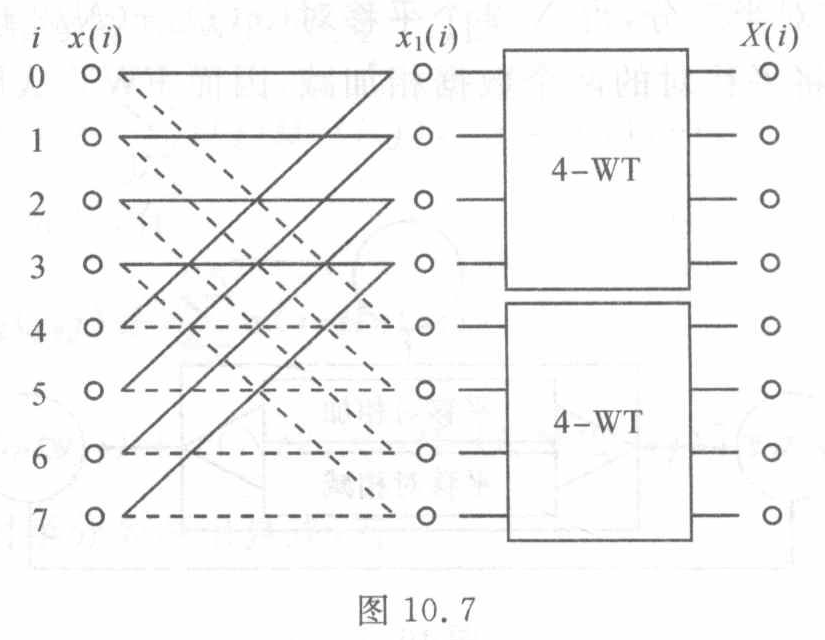
\includegraphics[width=0.85\linewidth,height=\textheight,keepaspectratio,alt={图 10.7（原图裁切）：8-WT 经第一步化成两个 4-WT}]{../assets/ch10/fig-10-7.png}

图 10.7

\begin{quote}
图中文字与图意（转录）：从左到右的列标为 \(i\)、\(x(i)\)、\(x_1(i)\)、\(X(i)\)。\(i\) 的行标为 0、1、2、3、4、5、6、7；两组模块均标为 4-WT。第一个加工阶段将行对 \((0,4)\)、\((1,5)\)、\((2,6)\)、\((3,7)\) 相加减，所得 \(x_1(i)\) 的前四项、后四项分别接入一个 4-WT，右端输出 \(X(i)\)。
\end{quote}

\textbf{步 2}　对 2 个 4-WT 分别施行 \(N=4\) 的二分手续（10.4.2），即

\[
\begin{aligned}
x_2(0)&=x_1(0)+x_1(2),& x_2(2)&=x_1(0)-x_1(2),\\
x_2(1)&=x_1(1)+x_1(3),& x_2(3)&=x_1(1)-x_1(3)
\end{aligned}
\]

与

\[
\begin{aligned}
x_2(4)&=x_1(4)+x_1(6),& x_2(6)&=x_1(4)-x_1(6),\\
x_2(5)&=x_1(5)+x_1(7),& x_2(7)&=x_1(5)-x_1(7),
\end{aligned}
\]

进一步加工出关于数据 \(\{x_2(j)\}\) 的 4 个 2-WT。这一演化步如图 10.8 所示。

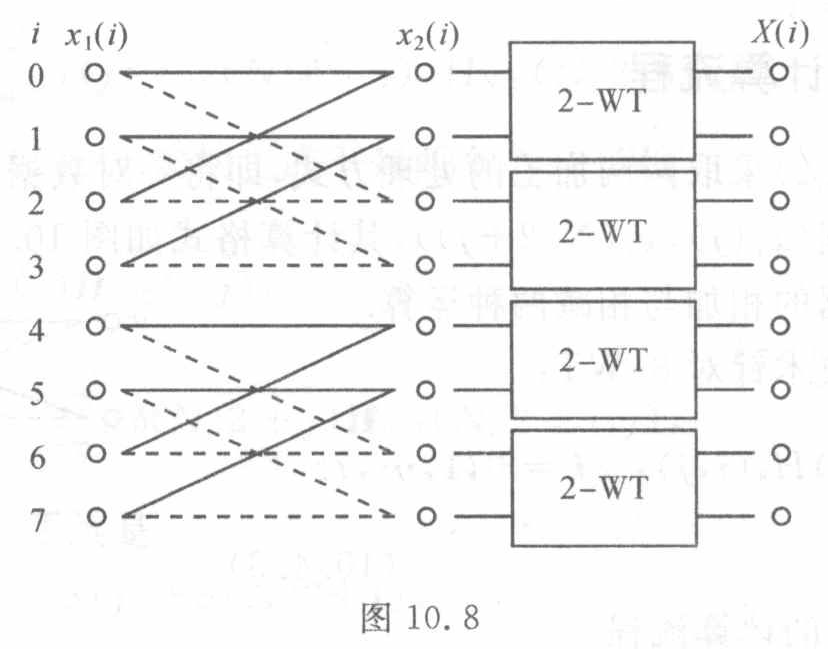
\includegraphics[width=0.85\linewidth,height=\textheight,keepaspectratio,alt={图 10.8（原图裁切）：两个 4-WT 经第二步化成四个 2-WT}]{../assets/ch10/fig-10-8.png}

图 10.8

\begin{quote}
图中文字与图意（转录）：从左到右的列标为 \(i\)、\(x_1(i)\)、\(x_2(i)\)、\(X(i)\)。\(i\) 的行标为 0、1、2、3、4、5、6、7；四组模块均标为 2-WT。该阶段将行对 \((0,2)\)、\((1,3)\)、\((4,6)\)、\((5,7)\) 相加减，所得 \(x_2(i)\) 每两项接入一个 2-WT，右端输出 \(X(i)\)。
\end{quote}

\textbf{步 3}　再对每个 2-WT 分别施行二分手续，即

\href{../../source-images/pdf-274.jpeg}{原页}

\[
\begin{aligned}
x_3(0)&=x_2(0)+x_2(1),& x_3(1)&=x_2(0)-x_2(1),\\
x_3(2)&=x_2(2)+x_2(3),& x_3(3)&=x_2(2)-x_2(3),\\
x_3(4)&=x_2(4)+x_2(5),& x_3(5)&=x_2(4)-x_2(5),\\
x_3(6)&=x_2(6)+x_2(7),& x_3(7)&=x_2(6)-x_2(7).
\end{aligned}
\]

加工得出关于数据 \(\{x_3(i)\}\) 的 8 个 1-WT，即得所求结果：

\[
X(i)=x_3(i),\quad i=0,1,\cdots,7.
\]

上述算法 FWT，其计算模型与输入数据同步进行加工，在将计算模型从 8-WT 加工成 1-WT 的同时，输入数据被加工成输出结果 \(\{X(i)\}\)。综合上述各步即得 FWT 的数据加工流程图 10.9。

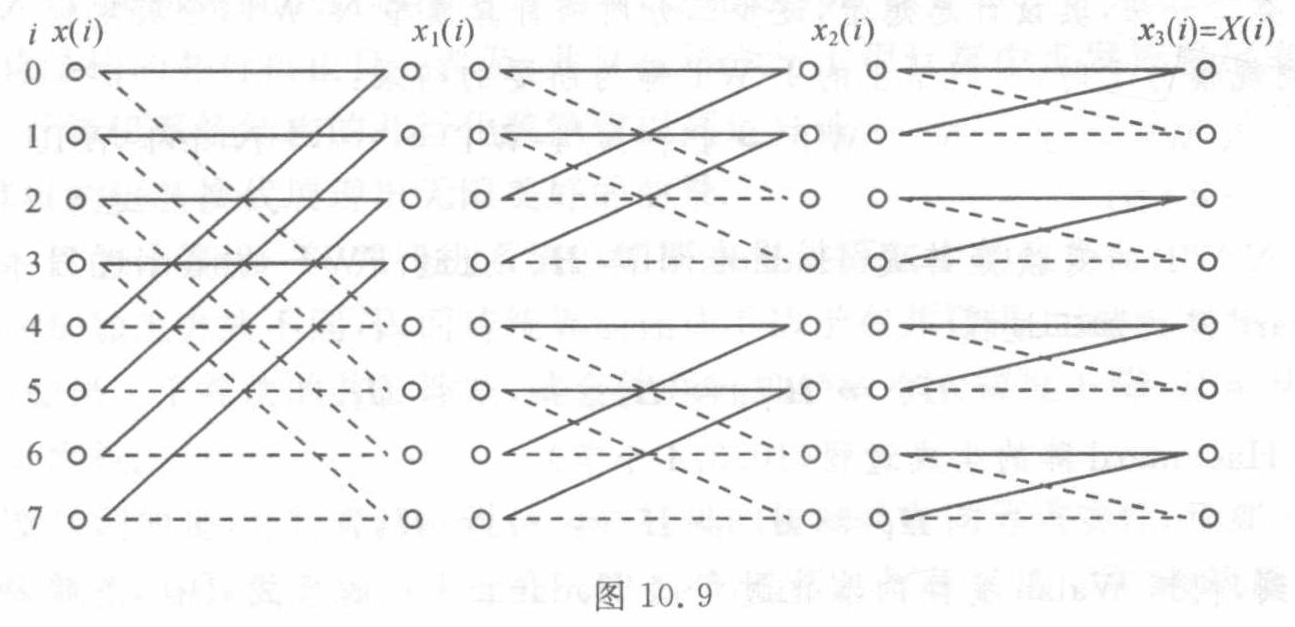
\includegraphics[width=0.85\linewidth,height=\textheight,keepaspectratio,alt={图 10.9（原图裁切）：8-WT 的完整数据加工流程}]{../assets/ch10/fig-10-9.png}

图 10.9

\begin{quote}
图中文字与图意（转录）：列标依次为 \(i\)、\(x(i)\)、\(x_1(i)\)、\(x_2(i)\)、\(x_3(i)=X(i)\)，行标为 0、1、2、3、4、5、6、7。第一阶段配对 \((0,4)\)、\((1,5)\)、\((2,6)\)、\((3,7)\)；第二阶段配对 \((0,2)\)、\((1,3)\)、\((4,6)\)、\((5,7)\)；第三阶段配对 \((0,1)\)、\((2,3)\)、\((4,5)\)、\((6,7)\)。每对按图 10.6 的实线相加、虚线相减计算，三步后由 \(x_3(i)\) 得到 \(X(i)\)。
\end{quote}

\subsubsection{10.4.4　FWT 的算法实现}\label{fwt-ux7684ux7b97ux6cd5ux5b9eux73b0}

回头考察一般形式的 Walsh 变换 \(N\)-WT（10.4.1）。仍设 \(N=2^n\)，\(n\) 为正整数。前已指出，其快速算法设计分 \(n=\log_2N\) 步，每一步将计算问题的规模减半。记 \(N_k=N/2^k\)。快速 Walsh 变换 FWT 的第 \(k\) 步将所给 \(N\)-WT 化归为 \(2^k\) 个 \(N_k\)-WT，其输入数据 \(x_k(i)\) 被分割成 \(2^k\) 段，每段含有 \(N_k\) 个数据，具体地说，其 \(l\)（\(l=1,2,\cdots,2^k\)）段数据为

\[
x_k((l-1)N_k+j),\quad j=0,1,\cdots,N_k-1.
\]

这样，二分过程的第 \(k\) 步是先将 \(k-1\) 步生成的数据段

\[
x_{k-1}((l-1)N_{k-1}+j),\quad j=0,1,\cdots,N_{k-1}-1
\]

再对半切成两部分，其前半部分与后半部分分别是

\[
x_{k-1}((l-1)N_{k-1}+j);\quad x_{k-1}((l-1)N_{k-1}+N_k+j),\quad j=0,1,\cdots,N_k-1.
\]

然后将这两组数据按式（10.4.2）进行加工，结果有

\[
\begin{gathered}
\begin{cases}
x_k((l-1)N_{k-1}+j)=x_{k-1}((l-1)N_{k-1}+j)+x_{k-1}((l-1)N_{k-1}+N_k+j),\\
x_k((l-1)N_{k-1}+N_k+j)=x_{k-1}((l-1)N_{k-1}+j)-x_{k-1}((l-1)N_{k-1}+N_k+j),
\end{cases}\\
j=0,1,\cdots,N_k-1;\quad l=1,2,\cdots,2^k.
\end{gathered}
\tag{10.4.4}
\]

\begin{quote}
校注（agent 补充，CH10-E004）：式（10.4.4）原印 \(l=1,2,\cdots,2^k\)，上文照录。此式用 \((l-1)N_{k-1}\) 定位第 \(k-1\) 步的数据段，该步只有 \(2^{k-1}\) 段，因此上限应为 \(2^{k-1}\)。例如 \(N=8,k=1\) 时，按原印取 \(l=2\) 会访问从索引 8 开始的数据，越过 \(0,\ldots,7\)。本页前文用于描述第 \(k\) 步结果分段数的 \(2^k\) 则正确。下一页算法 10.1 引用此式，也受该范围疑误影响。\href{../assets/ch10/erratum-p274-range.png}{原式放大裁片}。
\end{quote}

\href{../../source-images/pdf-275.jpeg}{原页}

这就是第 \(k\) 步所要施行的二分手续。反复施行这种二分手续即得所求的结果。于是有下列快速 Walsh 变换 FWT（算法 10.1）。

\textbf{算法 10.1}　令 \(x_0(i)=x(i)\)，\(i=0,1,\cdots,N-1\)，对 \(k=1,2,\cdots\) 直到 \(n=\log_2N\) 执行算式（10.4.4），结果有

\[
X(i)=x_n(i),\quad i=0,1,\cdots,N-1.
\]

\subsection{小结}\label{ux5c0fux7ed3}

本章阐述快速 Walsh 变换 FWT 的设计机理与设计方法。可以看到，FWT 本质上是一类二分法，其设计思想是，逐步二分所给计算模型 \(N\)-WT，令其规模 \(N\) 逐次减半，直到规模为 1 时，所归结出的 1-WT 即为所要的结果：

\[
\underset{\text{（计算模型）}}{N\text{-WT}}\Rightarrow2\text{ 个 }N/2\text{-WT}\Rightarrow4\text{ 个 }N/4\text{-WT}\Rightarrow\cdots\Rightarrow\underset{\text{（所求结果）}}{N\text{ 个 }1\text{-WT}}.
\]

注意到 \(N\)-WT 的变换矩阵是 Hadamard 阵 \(H_N\)，上述 FWT 的设计过程本质上是 Hadamard 阵的加工过程

\[
H_N\Rightarrow H_{N/2}\Rightarrow H_{N/4}\Rightarrow\cdots\Rightarrow H_1.
\]

再对比 Hadamard 阵的生成过程（10.3.4 小节）

\[
H_1\Rightarrow H_2\Rightarrow H_4\Rightarrow\cdots\Rightarrow H_N,
\]

可以看到，快速 Walsh 变换的演化过程同 Hadamard 阵的生成过程，它们两者互为反过程。如果后者视为\textbf{进化过程}（矩阵阶数逐步倍增），那么前者则是\textbf{退化过程}（矩阵阶数逐次减半）。在适当定义``规模''的前提下，它们两者全都从属于二分演化模式。

Walsh 分析处处都渗透了对立统一的辩证思维。

正因为 Walsh 函数具有极度的数学美，正由于 Walsh 分析展现了一种新的思维方式，因而在 Walsh 分析的基础上可以开展许多重要的研究。

快速 Walsh 变换是快速变换的一个重要的组成部分。运用变异技术，基于 Walsh 变换可以派生出其他种种快速变换，诸如 Haar 变换、斜变换、Hartly 变换等等，从而实现快速变换方法的大统一。

Walsh 分析有着广泛的应用前景。然而更为重要的是，它展现了一种新的数学方法------\textbf{演化数学方法}。

宇宙是演化的，生物是演化的。时至今日，辩证法关于发展变化的观点，即事物从低级到高级不断演化的观点，已经被科学界认为是无须论证的常识了。

Walsh 函数的演化分析用数学语言表述了这种``常识''。

Walsh 函数的演化分析无疑是新的数学革命即将爆发的先兆。还是 Harmuth 有远见：\textbf{Walsh 分析的研究将导致一场数学革命，就像 17、18 世纪的微积分那样。}

\subsection{本节覆盖原页的校注记录}\label{ux672cux8282ux8986ux76d6ux539fux9875ux7684ux6821ux6ce8ux8bb0ux5f55}

下列记录按原页关联，含同页相邻小节的校注；计算时同时读取上文校注和完整原页。

\begin{itemize}
\tightlist
\item
  \texttt{CH10-E001}：原书 PDF 页 271
\item
  \texttt{CH10-E002}：原书 PDF 页 270
\item
  \texttt{CH10-E003}：原书 PDF 页 272
\item
  \texttt{CH10-E004}：原书 PDF 页 274
\end{itemize}

\end{document}
